
%\documentclass[11pts,a4paper,amsmath,amssymb,floatfix]{article}%{report}%{book}
\documentclass[12pts,a4paper,amsmath,amssymb,floatfix]{article}%{report}%{book}
\usepackage{graphicx,wrapfig,pdfpages}% Include figure files
%\usepackage{dcolumn,enumerate}% Align table columns on decimal point
\usepackage{enumerate,enumitem}% Align table columns on decimal point
\usepackage{bm,dpfloat}% bold math
\usepackage[pdftex,bookmarks,colorlinks=true,urlcolor=rltblue,citecolor=blue]{hyperref}
\usepackage{amsfonts,amsmath,amssymb,stmaryrd,indentfirst}
\usepackage{times,psfrag}
\usepackage{natbib}
\usepackage{color}
\usepackage{units}
\usepackage{rotating}
\usepackage{multirow}


\usepackage{pifont}
\usepackage{subfigure}
\usepackage{subeqnarray}
\usepackage{ifthen}

\usepackage{supertabular}
\usepackage{moreverb}
\usepackage{listings}
\usepackage{palatino}
%\usepackage{doi}
\usepackage{longtable}
\usepackage{float}
\usepackage{perpage}
\MakeSorted{figure}
%\usepackage{pdflscape}


%\usepackage{booktabs}
%\newcommand{\ra}[1]{\renewcommand{\arraystretch}{#1}}


\definecolor{rltblue}{rgb}{0,0,0.75}


%\usepackage{natbib}
\usepackage{fancyhdr} %%%%
\pagestyle{fancy}%%%%
% with this we ensure that the chapter and section
% headings are in lowercase
%%%%\renewcommand{\chaptermark}[1]{\markboth{#1}{}}
\renewcommand{\sectionmark}[1]{\markright{\thesection\ #1}}
\fancyhf{} %delete the current section for header and footer
\fancyhead[LE,RO]{\bfseries\thepage}
\fancyhead[LO]{\bfseries\rightmark}
\fancyhead[RE]{\bfseries\leftmark}
\renewcommand{\headrulewidth}{0.5pt}
% make space for the rule
\fancypagestyle{plain}{%
\fancyhead{} %get rid of the headers on plain pages
\renewcommand{\headrulewidth}{0pt} % and the line
}

\def\newblock{\hskip .11em plus .33em minus .07em}
\usepackage{color}

%\usepackage{makeidx}
%\makeindex

\setlength\textwidth      {16.cm}
\setlength\textheight     {22.6cm}
\setlength\oddsidemargin  {-0.3cm}
\setlength\evensidemargin {0.3cm}

\setlength\headheight{14.49998pt} 
\setlength\topmargin{0.0cm}
\setlength\headsep{1.cm}
\setlength\footskip{1.cm}
\setlength\parskip{0pt}
\setlength\parindent{0pt}


%%%
%%% Headers and Footers
\lhead[] {\text{\small{EG501J -- Geothermal Energy}}} 
\rhead[] {{\text{\small{Tutorial 02b}}}}
%\chead[] {\text{\small{Session 2012/13}}} 
\lfoot[]{Dr Jeff Gomes}
%\cfoot[\thepage]{\thepage}
\rfoot[\text{\small{\thepage}}]{\thepage}
\renewcommand{\headrulewidth}{0.8pt}


%%%
%%% space between lines
%%%
\renewcommand{\baselinestretch}{1.5}

\newenvironment{VarDescription}[1]%
  {\begin{list}{}{\renewcommand{\makelabel}[1]{\textbf{##1:}\hfil}%
    \settowidth{\labelwidth}{\textbf{#1:}}%
    \setlength{\leftmargin}{\labelwidth}\addtolength{\leftmargin}{\labelsep}}}%
  {\end{list}}

%%%%%%%%%%%%%%%%%%%%%%%%%%%%%%%%%%%%%%%%%%%
%%%%%%                              %%%%%%%
%%%%%%      NOTATION SECTION        %%%%%%%
%%%%%%                              %%%%%%%
%%%%%%%%%%%%%%%%%%%%%%%%%%%%%%%%%%%%%%%%%%%

% Text abbreviations.
\newcommand{\ie}{{\em{i.e., }}}
\newcommand{\eg}{{\em{e.g., }}}
\newcommand{\cf}{{\em{cf., }}}
\newcommand{\wrt}{with respect to}
\newcommand{\lhs}{left hand side}
\newcommand{\rhs}{right hand side}
% Commands definining mathematical notation.

% This is for quantities which are physically vectors.
\renewcommand{\vec}[1]{{\mbox{\boldmath$#1$}}}
% Physical rank 2 tensors
\newcommand{\tensor}[1]{\overline{\overline{#1}}}
% This is for vectors formed of the value of a quantity at each node.
\newcommand{\dvec}[1]{\underline{#1}}
% This is for matrices in the discrete system.
\newcommand{\mat}[1]{\mathrm{#1}}


\DeclareMathOperator{\sgn}{sgn}
\newtheorem{thm}{Theorem}[section]
\newtheorem{lemma}[thm]{Lemma}

%\newcommand\qed{\hfill\mbox{$\Box$}}
\newcommand{\re}{{\mathrm{I}\hspace{-0.2em}\mathrm{R}}}
\newcommand{\inner}[2]{\langle#1,#2\rangle}
\renewcommand\leq{\leqslant}
\renewcommand\geq{\geqslant}
\renewcommand\le{\leqslant}
\renewcommand\ge{\geqslant}
\renewcommand\epsilon{\varepsilon}
\newcommand\eps{\varepsilon}
\renewcommand\phi{\varphi}
\newcommand{\bmF}{\vec{F}}
\newcommand{\bmphi}{\vec{\phi}}
\newcommand{\bmn}{\vec{n}}
\newcommand{\bmns}{{\textrm{\scriptsize{\boldmath $n$}}}}
\newcommand{\bmi}{\vec{i}}
\newcommand{\bmj}{\vec{j}}
\newcommand{\bmk}{\vec{k}}
\newcommand{\bmx}{\vec{x}}
\newcommand{\bmu}{\vec{u}}
\newcommand{\bmv}{\vec{v}}
\newcommand{\bmr}{\vec{r}}
\newcommand{\bma}{\vec{a}}
\newcommand{\bmg}{\vec{g}}
\newcommand{\bmU}{\vec{U}}
\newcommand{\bmI}{\vec{I}}
\newcommand{\bmq}{\vec{q}}
\newcommand{\bmT}{\vec{T}}
\newcommand{\bmM}{\vec{M}}
\newcommand{\bmtau}{\vec{\tau}}
\newcommand{\bmOmega}{\vec{\Omega}}
\newcommand{\pp}{\partial}
\newcommand{\kaptens}{\tensor{\kappa}}
\newcommand{\tautens}{\tensor{\tau}}
\newcommand{\sigtens}{\tensor{\sigma}}
\newcommand{\etens}{\tensor{\dot\epsilon}}
\newcommand{\ktens}{\tensor{k}}
\newcommand{\half}{{\textstyle \frac{1}{2}}}
\newcommand{\tote}{E}
\newcommand{\inte}{e}
\newcommand{\strt}{\dot\epsilon}
\newcommand{\modu}{|\bmu|}
% Derivatives
\renewcommand{\d}{\mathrm{d}}
\newcommand{\D}{\mathrm{D}}
\newcommand{\ddx}[2][x]{\frac{\d#2}{\d#1}}
\newcommand{\ddxx}[2][x]{\frac{\d^2#2}{\d#1^2}}
\newcommand{\ddt}[2][t]{\frac{\d#2}{\d#1}}
\newcommand{\ddtt}[2][t]{\frac{\d^2#2}{\d#1^2}}
\newcommand{\ppx}[2][x]{\frac{\partial#2}{\partial#1}}
\newcommand{\ppxx}[2][x]{\frac{\partial^2#2}{\partial#1^2}}
\newcommand{\ppt}[2][t]{\frac{\partial#2}{\partial#1}}
\newcommand{\pptt}[2][t]{\frac{\partial^2#2}{\partial#1^2}}
\newcommand{\DDx}[2][x]{\frac{\D#2}{\D#1}}
\newcommand{\DDxx}[2][x]{\frac{\D^2#2}{\D#1^2}}
\newcommand{\DDt}[2][t]{\frac{\D#2}{\D#1}}
\newcommand{\DDtt}[2][t]{\frac{\D^2#2}{\D#1^2}}
% Norms
\newcommand{\Ltwo}{\ensuremath{L_2} }
% Basis functions
\newcommand{\Qone}{\ensuremath{Q_1} }
\newcommand{\Qtwo}{\ensuremath{Q_2} }
\newcommand{\Qthree}{\ensuremath{Q_3} }
\newcommand{\QN}{\ensuremath{Q_N} }
\newcommand{\Pzero}{\ensuremath{P_0} }
\newcommand{\Pone}{\ensuremath{P_1} }
\newcommand{\Ptwo}{\ensuremath{P_2} }
\newcommand{\Pthree}{\ensuremath{P_3} }
\newcommand{\PN}{\ensuremath{P_N} }
\newcommand{\Poo}{\ensuremath{P_1P_1} }
\newcommand{\PoDGPt}{\ensuremath{P_{-1}P_2} }

\newcommand{\metric}{\tensor{M}}
\newcommand{\configureflag}[1]{\texttt{#1}}

% Units
\newcommand{\m}[1][]{\unit[#1]{m}}
\newcommand{\km}[1][]{\unit[#1]{km}}
\newcommand{\s}[1][]{\unit[#1]{s}}
\newcommand{\invs}[1][]{\unit[#1]{s}\ensuremath{^{-1}}}
\newcommand{\ms}[1][]{\unit[#1]{m\ensuremath{\,}s\ensuremath{^{-1}}}}
\newcommand{\mss}[1][]{\unit[#1]{m\ensuremath{\,}s\ensuremath{^{-2}}}}
\newcommand{\K}[1][]{\unit[#1]{K}}
\newcommand{\PSU}[1][]{\unit[#1]{PSU}}
\newcommand{\Pa}[1][]{\unit[#1]{Pa}}
\newcommand{\kg}[1][]{\unit[#1]{kg}}
\newcommand{\rads}[1][]{\unit[#1]{rad\ensuremath{\,}s\ensuremath{^{-1}}}}
\newcommand{\kgmm}[1][]{\unit[#1]{kg\ensuremath{\,}m\ensuremath{^{-2}}}}
\newcommand{\kgmmm}[1][]{\unit[#1]{kg\ensuremath{\,}m\ensuremath{^{-3}}}}
\newcommand{\Nmm}[1][]{\unit[#1]{N\ensuremath{\,}m\ensuremath{^{-2}}}}

% Dimensionless numbers
\newcommand{\dimensionless}[1]{\mathrm{#1}}
\renewcommand{\Re}{\dimensionless{Re}}
\newcommand{\Ro}{\dimensionless{Ro}}
\newcommand{\Fr}{\dimensionless{Fr}}
\newcommand{\Bu}{\dimensionless{Bu}}
\newcommand{\Ri}{\dimensionless{Ri}}
\renewcommand{\Pr}{\dimensionless{Pr}}
\newcommand{\Pe}{\dimensionless{Pe}}
\newcommand{\Ek}{\dimensionless{Ek}}
\newcommand{\Gr}{\dimensionless{Gr}}
\newcommand{\Ra}{\dimensionless{Ra}}
\newcommand{\Sh}{\dimensionless{Sh}}
\newcommand{\Sc}{\dimensionless{Sc}}


% Journals
\newcommand{\IJHMT}{{\it International Journal of Heat and Mass Transfer}}
\newcommand{\NED}{{\it Nuclear Engineering and Design}}
\newcommand{\ICHMT}{{\it International Communications in Heat and Mass Transfer}}
\newcommand{\NET}{{\it Nuclear Engineering and Technology}}
\newcommand{\HT}{{\it Heat Transfer}}   
\newcommand{\IJHT}{{\it International Journal for Heat Transfer}}

\newcommand{\frc}{\displaystyle\frac}
\newcommand{\red}{\textcolor{red}}
 
\newlist{ExList}{enumerate}{1}
\setlist[ExList,1]{label={\bf Example 1.} {\bf \arabic*}}

\newlist{ProbList}{enumerate}{1}
\setlist[ProbList,1]{label={\bf Problem 1.} {\bf \arabic*}}

%%%%%%%%%%%%%%%%%%%%%%%%%%%%%%%%%%%%%%%%%%%
%%%%%%                              %%%%%%%
%%%%%% END OF THE NOTATION SECTION  %%%%%%%
%%%%%%                              %%%%%%%
%%%%%%%%%%%%%%%%%%%%%%%%%%%%%%%%%%%%%%%%%%%


% Cause numbering of subsubsections. 
%\setcounter{secnumdepth}{8}
%\setcounter{tocdepth}{8}

\setcounter{secnumdepth}{4}%
\setcounter{tocdepth}{4}%


\begin{document}

A geothermal power plant operates under binary cycle technology with propane, C$_{3}$, as working fluid $\left(\text{with mass flow rate of 10 kg.s}^{-1}\right)$. The geothermal fluid is extracted  from the production well ($A$) at 35 kg.s$^{-1}$ and 120$^{\circ}$C. Thermal energy from the geothermal stream is transferred into the propane flow in the heat exchanger operating at 18 bar, resulting in a temperature of 70 $^{\circ}$C. A turbine isentropically expands the propane fluid to 0.75 bar. Calculate:
\begin{enumerate}
  \item Net work produced by the cycle;
  \item Heat removed from the working fluid through the condenser;
  \item Temperature of the geothermal fluid ($B$) before reinjection; 
\end{enumerate}
Assume that the heat capacity at constant pressure $\left(C_{p,w}\right)$ of the geothermal fluid is $4.18$ kJ.$\left(\text{kg.}^{\circ}\text{C}\right)^{-1}$.


\begin{center}
\includegraphics[width=15.0cm,height=12.0cm]{./Pics/GeothermalPowerGeneration}
\end{center}


\clearpage

\begin{center}
{\large {\bf Solution}}
\end{center}

Before we solve (1-3), we need to calculate the enthalpies of propane at each stage of the cycle:

\begin{enumerate}[label=\bfseries Stage \arabic*:]
%

\item At $P_{1}=18\text{ bar} \longrightarrow T_{\text{sat}}=52.3^{\circ}\text{C} < T_{1}\left(=70^{\circ}\text{C}\right)$, therefore, we can conclude that propane is at {\it superheated} state. From the superheated fluid table:
\begin{itemize}
  \item \red{$h_{1} = 561.8$ kJ.kg$^{-1}$};
  \item $s_{1} = 1.834$ kJ.$\left(\text{kg.K}\right)^{-1}$
\end{itemize}
%

\item In the turbine, propane is {\it isentropically} $\left(\text{i.e., } s_{2} = s_{1}\right)$ expanded from $P_{1}=18\text{ bar}$ to $P_{2}=0.75\text{ bar}$. During the expansion, the fluid is cooled and may undertake phase change (i.e., part of the vapour may be condensed producing droplets of liquid propane), and we need to assess the {\it quality} $\left(x_{2}\right)$ of the stream,
\begin{displaymath}
  x_{2} = \frc{s_{2}-s_{f}}{s_{g}-s_{f}} = \frc{1.834-(-0.085)}{1.841-(-0.085)} = 0.9964
\end{displaymath}

This indicates that the fluid is almost fully vaporised (99.64$\%$ of vapour). With the quality we can finally calculate the enthalpy of this stream,
\begin{displaymath}
  x_{2} = 0.9964 = \frc{h_{2}-h_{f}}{h_{g}-h_{f}} = \frc{h_{2} - (-19.5)}{412.8 - (-19.5)} \Longrightarrow \red{h_{2} = 411.24\; \text{kJ.kg}^{-1}} 
\end{displaymath} 
%
\item Propane is then {\bf fully condensated} (phase change from vapour to liquid) at {\it constant pressure} at the condenser, i.e., $P_{2}=P_{3}=0.75\text{ bar}$. Therefore, from the saturated fluid property table,
\begin{itemize}
   \item \red{$h_{3}$} = $h_{f}$ \red{$= -19.5 \text{ kJ.kg}^{-1}$};
   \item $s_{3} = s_{f} = -0.085\text{ kJ.}\left(\text{kg.K}\right)^{-1}$;
   \item $v_{3} = v_{f} = 1.698\times 10^{-3}\text{ m}^{3}\text{.kg}^{-1}$;
\end{itemize}
%

\item After being fully condensated, liquid propane is {\it isentropically compressed} in a pump and driven towards the heat exchanger. Assuming that there is \underline{no pressure drop} in the heat exchanger, we can conclude that $P_{4}=P_{1}=18\text{ bar}$. We can also assume that the liquid propane is incompressible (i.e., no change in volume as pressure is modified) and integrating the fundamental thermodynamic relation $dh = vdP$ from stage 3 to stage 4,
\begin{eqnarray}
   \red{h_{4}} &=& h_{3} + v_{3}\left(P_{4}-P_{3}\right) = -19.5\frc{kJ}{kg} + 1.698\times 10^{-3}\frc{m^{3}}{kg}\left(18-0.75\right)\text{bar}\times \frc{10^{5}\frc{kg}{m.s^{2}}}{1\text{ bar}} \times \frc{10^{-3}\frc{kJ}{kg}}{1\frc{m^{2}}{s^{2}}}
 \nonumber \\
              &=& \red{-16.57\frc{kJ}{kg}} \nonumber
\end{eqnarray} 
%
\end{enumerate}

Now that we obtained all enthalpies of the cycle, we can solve (1-3):
\begin{enumerate}
%
\item Net work:
\begin{eqnarray}
\red{\dot{W}_{\text{net}}} &=& \dot{W}_{\text{turbine}} + \dot{W}_{\text{pump}} = \dot{m}_{C_{3}}\left[\left(h_{2}-h_{1}\right) + \left(h_{4}-h_{3}\right)\right] \nonumber \\
                        &=& 10\frc{kg}{s}\left[\left(411.24-561.8\right) + \left(-16.57-(-19.50)\right)\right]\frc{kJ}{kg} = \red{-1476.3\;\frc{kJ}{s}} \nonumber
\end{eqnarray}
Thus \red{$\sim$ 1.48 MW} of power were \underline{produced by the cycle}.
%
\item The thermal energy that can be (potentially) used in district heating (or in industrial facilities or waste in the environment) is,
\begin{eqnarray}
 \red{\dot{Q}_{\text{condenser}}} &=& \dot{m}_{C_{3}}\left(h_{3}-h_{2}\right) = 10\frc{kg}{s}\left(-19.5-411.24\right)\frc{kJ}{kg} \nonumber \\
                             &=& \red{-4307.4\;\frc{kJ}{s}} \nonumber
\end{eqnarray}
Thus the cycle generated \red{$\sim$4.3 MW} of heating that can be effectively used.
%

\item In order to calculate the temperature of the geothermal fluid before reinjection, we first need to calculate the {\it heat absorbed by propane in the heat exchanger},
\begin{eqnarray}
\dot{Q}_{\text{absorbed}} &=& \dot{m}_{C_{3}}\left(h_{1}-h_{4}\right) = 10\frc{kg}{s}\left(561.8-(-16.57)\right)\frc{kJ}{kg} \nonumber \\
                      &=& 5783.7\; \frc{kJ}{s} \nonumber 
\end{eqnarray}
Assuming that no heat is lost in the heat exchanger through the boundaries to the surroundings, the total energy balance is $\dot{Q}_{\text{absorbed}}+\dot{Q}_{\text{released}} = 0$, thus
\begin{eqnarray}
 \dot{Q}_{\text{released}} &=& \dot{m}_{w}C_{p,w}\left(T_{w}^{\text{out}}-T_{w}^{\text{in}}\right) \nonumber \\
 -5783.7 \frc{kJ}{s}    &=& 35\;\frc{kg}{s} \times 4.18\;\frc{kJ}{kg.^{\circ}C}\times \left(T_{w}^{\text{out}}-120\right)^{\circ}C \nonumber \\
 \red{T_{w}^{\text{out}}}   &=& \red{80.47^{\circ}C} \nonumber
\end{eqnarray}
The geothermal fluid will need to be cooled before reinjection as the temperature is probably too large to comply with environmental laws.   
%
\end{enumerate} 



%{
%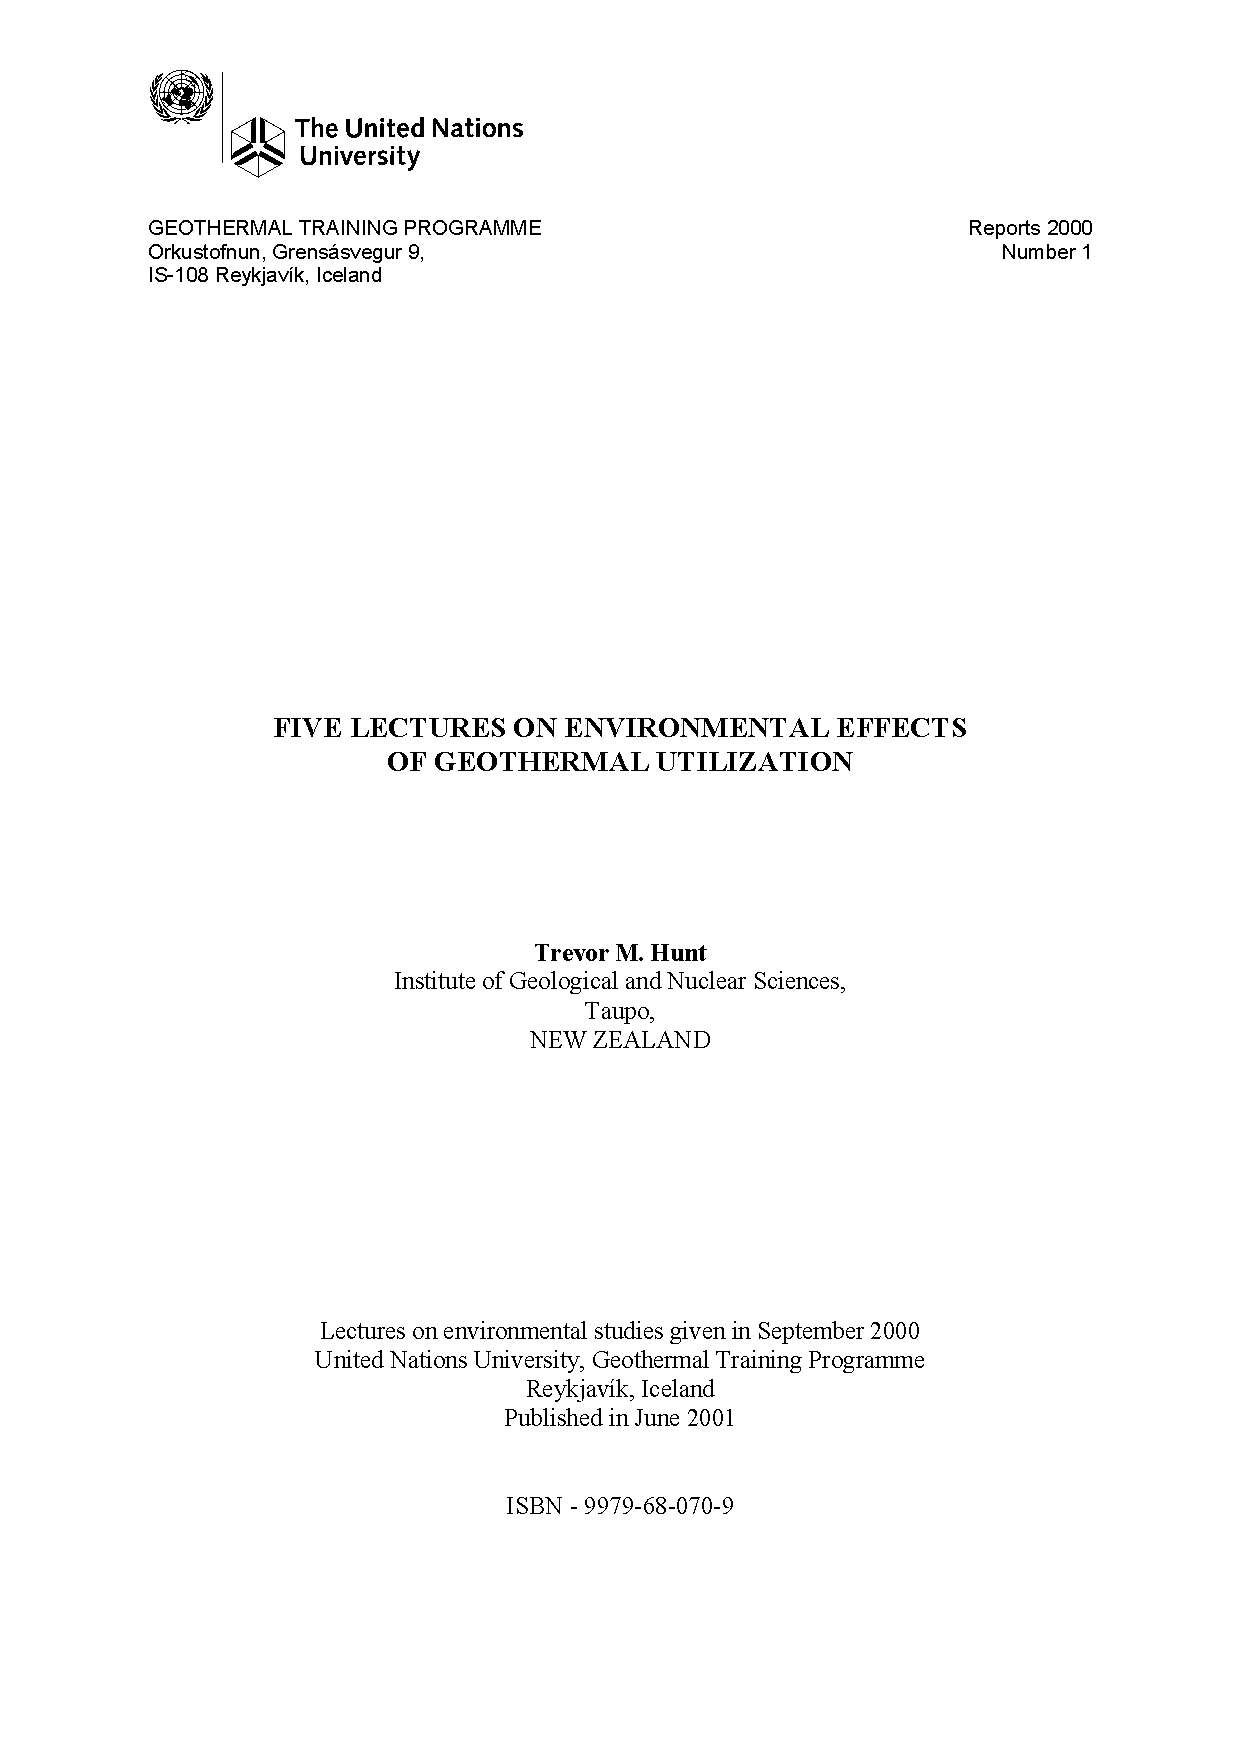
\includepdf[pages=-,fitpaper, angle=0]{./HuntSelect.pdf}
%}

\end{document}
